\section*{\RU{Предисловие}\EN{Preface}}

\RU{Здесь (будет) немного моих заметок о \gls{reverse engineering} на русском языке для начинающих, 
для тех кто хочет научиться понимать создаваемый \CCpp компиляторами код для x86 (коего, 
практически, больше всего остального) и ARM.}
\EN{Here are some of my notes in English for beginners about \gls{reverse engineering}
who would like to learn to understand x86 (which accounts for almost
all executable software in the world) and ARM code created by \CCpp compilers.}

\RU{У термина ``\gls{reverse engineering}'' несколько популярных значений: 
1) исследование скомпилированных
программ; 2) сканирование трехмерной модели для последующего копирования;
3) восстановление структуры СУБД. Настоящий сборник заметок
связан с первым значением}
\EN{There are several popular meanings of the term ``\gls{reverse engineering}'': 
1) reverse engineering of software: researching compiled programs;
2) 3D model scanning and reworking in order to make a copy of it;
3) recreating \ac{DBMS} structure.
This book is related to the first meaning.}

\ifx\LITE\undefined
\subsection*{\RU{Рассмотренные темы}\EN{Topics discussed}}

x86/x64, ARM/ARM64, MIPS.

\subsection*{\RU{Затронутые темы}\EN{Topics touched}}

\oracle (\ref{oracle}),
Itanium (\ref{itanium}),
\RU{донглы для защиты от копирования}\EN{copy-protection dongles} (\ref{dongles}), 
LD\_PRELOAD (\ref{ld_preload}),
\RU{переполнение стека}\EN{stack overflow}, 
\ac{ELF},
\RU{формат файла PE в win32}\EN{win32 PE file format} (\ref{win32_pe}),
x86-64 (\ref{x86-64}),
\RU{критические секции}\EN{critical sections} (\ref{critical_sections}),
\RU{сисколлы}\EN{syscalls} (\ref{syscalls}), 
\ac{TLS},
\RU{адресно-независимый код}\EN{position-independent code} (\ac{PIC}) (\ref{sec:PIC}), 
profile-guided optimization (\ref{PGO}),
C++ STL (\ref{cpp_STL}),
OpenMP (\ref{openmp}),
SEH (\ref{sec:SEH}).
\fi

\subsection*{\RU{Еще кое-что}\EN{Notes}}

\newcommand{\FNURLREDDIT}{\footnote{\href{http://go.yurichev.com/17027}{reddit}}}

\EN{Why one should learn assembly language these days?}
\RU{Зачем в наше время нужно изучать язык ассемблера?}
\EN{Unless you are OS developer, you probably don't need to write in assembly: 
modern compilers perform optimizations much better than humans do.}
\RU{Если вы не разработчик OS, вам наверное не нужно писать на ассемблере:
современные компиляторы оптимизируют код намного лучше человека}
\footnote{\RU{Очень хороший текст на эту тему}\EN{A very good text about this topic}: \cite{AgnerFog}}.
\EN{Also, modern \ac{CPU}s are very complex devices and assembly knowledge would 
not help you understand its internals.}
\RU{Современные \ac{CPU} это также крайне сложные устройства, и знание ассемблера вряд ли
поможет узнать его внутренности.}
\EN{That said, there are at least two areas where a good understanding of assembly may help:
first, security/malware research. Second, gaining a better understanding of your compiled code
while debugging.}
\RU{Но все-таки остается по крайней мере две области, где знание ассемблера может хорошо
помочь:
1) исследование malware (\IT{зловредов}) в целях security research; 2) лучшее понимание
вашего скомпилированного кода в процессе отладки.}

\EN{Therefore, this book is intended for those who want to understand assembly language rather 
than to write in it, which is why there are many examples of compiler output.}
\RU{Таким образом, эта книга предназначена для тех, кто хочет скорее понимать ассемблер,
нежели писать на нем, и вот почему здесь масса примеров связанных с результатами
работы компиляторов.}\\
\\
\RU{Как можно найти работу reverse engineer-а}\EN{How would one find a reverse engineering job}? \\
\RU{На reddit, посвященному RE\FNURLREDDIT, время от времени бывают hiring thread}
\EN{There are hiring threads that appear from time to time on reddit devoted to RE\FNURLREDDIT}
(\href{http://go.yurichev.com/17333}{2013 Q3}, 
\href{http://go.yurichev.com/17334}{2014}).
\RU{Посмотрите там}\EN{Try looking there}.
\EN{A somewhat related hiring thread can be found in the ``netsec'' subreddit}\RU{В смежном субреддите ``netsec'' имеется похожий тред}: 
\href{http://go.yurichev.com/17335}{2014 Q2}.\\
\\
\RU{Куда пойти учиться в Украине?
\begin{itemize}
\item НТУУ <<КПИ>>: ``Аналіз програмного коду та бінарних вразливостей'' \url{http://go.yurichev.com/17336}.
\item \url{http://go.yurichev.com/17337} (факультативы).
\end{itemize}}

\subsection*{\RU{Об авторе}\EN{About the author}}

\begin{tabularx}{\textwidth}{ l X }

\raisebox{-\totalheight}{
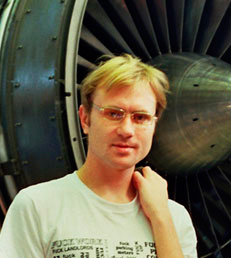
\includegraphics[scale=0.60]{Dennis_Yurichev.jpg}
}

&
\RU{Денис Юричев ~--- опытный reverse engineer и программист.
С его резюме можно ознакомиться на его сайте}
\EN{Dennis Yurichev is an experienced reverse engineer and programmer.
His CV is available on his website}\footnote{\href{http://go.yurichev.com/17141}{yurichev.com}}. \\
% FIXME: no link. \tablefootnote doesn't work
\end{tabularx}

\subsection*{\RU{Благодарности}\EN{Thanks}}

\RU{Тем, кто много помогал мне отвечая на массу вопросов}\EN{For patiently answering all my questions}:
\HERMIT, \RU{Слава ''Avid'' Казаков}\EN{Slava ''Avid'' Kazakov}.

\RU{Тем, кто присылал замечания об ошибках и неточностях}\EN{For sending me notes
about mistakes and inaccuracies}:
\RU{Станислав ''Beaver'' Бобрицкий, Александр Лысенко}
\EN{Stanislav ''Beaver'' Bobrytskyy, Alexander Lysenko}, Shell Rocket, Zhu Ruijin, Changmin Heo.

\RU{Просто помогали разными способами}\EN{For helping me in other ways}:
\RU{Андрей Зубинский}\EN{Andrew Zubinski}, 
Arnaud Patard (rtp \RU{на}\EN{on} \#debian-arm IRC).

\RU{Переводчику на китайский язык}\EN{For translating to Chinese simplified}: Xian Chi.

\RU{Переводчику на корейский язык}\EN{For translating to Korean}: Byungho Min.

\RU{Корректорам}\EN{For proofreading}:
\RU{Александр ''Lstar'' Черненький}\EN{Alexander ''Lstar'' Chernenkiy},
\RU{Владимир Ботов}\EN{Vladimir Botov},
\RU{Андрей Бражук}\EN{Andrei Brazhuk},
\RU{Марк}\EN{Mark} ``Logxen'' \RU{Купер}\EN{Cooper},
Yuan Jochen Kang, Vasil Kolev.

\RU{И еще всем тем на github.com кто присылал замечания и коррективы}
\EN{Thanks also to all the folks on github.com who have contributed notes and corrections}.

\RU{Было использовано множество пакетов \LaTeX\: их авторов я также хотел бы поблагодарить}
\EN{Many \LaTeX\ packages were used: I would like to thank the authors as well}.

\subsection{\RU{Пожертвования}\EN{Donate}}
\label{sec:donate}

\RU{Как выясняется, быть (техническим) писателем требует много сил и работы}
\EN{As it turns out, (technical) writing takes a lot of effort and work}.

\RU{Эта книга является свободной, находится в свободном доступе, и доступна в виде исходных кодов}
\EN{This book is free, available freely and available in source code form}
\footnote{\href{http://go.yurichev.com/17089}{GitHub}} (LaTeX), 
\RU{и всегда будет оставаться таковой}\EN{and it will be so forever}.

\EN{It's also ad-free}\RU{Тут также нет рекламы}.

\RU{В мои текущие планы насчет этой книги входит добавление информации на эти темы}
\EN{My current plan for this book is to add lots of information about}:
PLANS\footnote{\href{http://go.yurichev.com/17090}{GitHub}}.

\RU{Если вы хотите, чтобы я продолжал свою работу и писал на эти темы,
вы можете рассмотреть идею пожертвования}
\EN{If you want me to continue writing on all these topics you may consider donating}.

\RU{Я писал эту книгу более года}\EN{I worked more than a year on this book}
\footnote{\RU{Самый первый коммит в git от марта 2013}\EN{Initial git commit from March 2013}: \\
\href{http://go.yurichev.com/17091}{GitHub}},
\RU{здесь более 800 страниц}\EN{there are more than 800 pages}.
\RU{Здесь как минимум $\approx 400$ \TeX-файлов, $\approx 150$ исходников на \CCpp, 
$\approx 470$ различных листингов, $\approx 160$ скриншотов}
\EN{There are at least $\approx 400$ \TeX-files, $\approx 150$ \CCpp source codes, 
$\approx 470$ various listings, $\approx 160$ screenshots}.

\RU{Цены на другие книги по этой же тематике на amazon.com колеблются в пределах от \$20 до \$50}
\EN{Price of other books on the same subject varies between \$20 and \$50 on amazon.com}.

\RU{Со способами пожертвовать деньги можно ознакомиться на странице}
\EN{Ways to donate are available on the page:} \href{http://go.yurichev.com/17011}{beginners.re}.

\RU{Имена всех жертвователей будут перечислены в книге}
\EN{Every donor's name will be included in the book}!
\RU{Жертвователи также имеют право просить меня дописывать в книгу что-то раньше, чем остальное}
\EN{Donors also have a right to ask me to rearrange items in my writing plan}.

\iffalse
\RU{Почему не попробовать издаться}\EN{Why not try to publish}?
\RU{Потому что это техническая литература, которая, как мне кажется,
не может быть закончена или быть замороженной в бумажном виде}
\EN{Because it's technical literature which, as I believe, cannot be finished or frozen in paper state}.
\RU{Такие технические справочники чем-то похожи на Wikipedia или библиотеку \ac{MSDN},
они могут развиваться бесконечно долго}
\EN{Such technical references akin to Wikipedia or \ac{MSDN} library.
They can evolve and grow indefinitely}.
\RU{Кто-то может сесть и, не отрываясь, написать всё от начала до конца, опубликовать это и забыть}
\EN{Someone can sit down and write everything from the begin to the end, publish it and forget about it}.
\RU{Как выясняется, это не я}\EN{As it turns out, it's not me}.
\RU{Каждый день меня посещают мысли вроде ``это было написано плохо, можно было бы и лучше написать'',
``это плохой пример, я знаю получше'',
``ещё одна вещь, которую я могу объяснить лучше и короче'' и т.д}
\EN{I have everyday thoughts like ``that was written badly and can be rewritten better'', 
``that was a bad example, I know a better one'', 
``that is also a thing I can explain better and shorter'', etc}.
\RU{Как можно увидеть в истории коммитов исходников этой книги,
я делаю много мелких изменений почти каждый день}
\EN{As you may see in commit history of this book's source code,
I make a lot of small changes almost every day}:
\href{http://go.yurichev.com/17092}{GitHub}.

\RU{Так что книга, наверное, будет в виде ``rolling release'', как говорят о дистрибутивах Linux вроде
Gentoo}
\EN{So the book will probably be a ``rolling release'' as they say about Linux distros like Gentoo}.
\RU{Без релизов (и дедлайнов) вообще, а постепенная разработка}
\EN{No fixed releases (and deadlines) at all, but continuous development}.
\RU{Я не знаю, сколько займет времени написать всё что я знаю. Может быть, 10 лет или больше}
\EN{I don't know how long it will take to write all I know. Maybe 10 years or more}.
\RU{Конечно, это не очень удобно для читателей, желающих стабильности,
но всё что я могу им предложить ~--- это файл ChangeLog}
\EN{Of course, it is not very convenient for readers who want something stable,
but all I can offer is a ChangeLog}
\footnote{\href{http://go.yurichev.com/17093}{GitHub}}
\RU{, служащий как секция ``что нового''}\EN{ file serving as a ``what's new'' section}.
\RU{Те, кому интересно, могут проверять его время от времени, или мой блог/twitter/facebook
\footnote{
\href{http://go.yurichev.com/17094}{blog.yurichev.com}
\href{http://go.yurichev.com/17021}{twitter}
\href{http://go.yurichev.com/17022}{facebook}
}}
\EN{Those who are interested may check it from time to time, or my blog/twitter/facebook
\footnote{
\href{http://go.yurichev.com/17094}{blog.yurichev.com}
\href{http://go.yurichev.com/17021}{twitter}
\href{http://go.yurichev.com/17022}{facebook}
}}.
\fi
\subsubsection*{\RU{Жертвователи}\EN{Donors}}

17 * \RU{аноним}\EN{anonymous}, 
2 * \RU{Олег Выговский}\EN{Oleg Vygovsky} (50+100 UAH), 
Daniel Bilar (\$50), 
James Truscott (\$4.5),
Luis Rocha (\$63), 
Joris van de Vis (\$127), 
Richard S Shultz (\$20), 
Jang Minchang (\$20), 
Shade Atlas (5 AUD), 
Yao Xiao (\$10),
Pawel Szczur (40 CHF), 
Justin Simms (\$20), 
Shawn the R0ck (\$27), 
Ki Chan Ahn (\$50), 
Triop AB (100 SEK), 
Ange Albertini (10 EUR),
\RU{Сергей Лукьянов}\EN{Sergey Lukianov} (300 RUR), 
Ludvig Gislason (200 SEK), 
Gérard Labadie (40 EUR), 
Sergey Volchkov (10 AUD),
Vankayala Vigneswararao (\$50),
Philippe Teuwen (\$4),
Martin Haeberli (\$10),
Victor Cazacov (5 EUR),
Tobias Sturzenegger (10 CHF),
Sonny Thai (\$15),
Bayna AlZaabi (\$75),
Redfive B.V. (25 EUR),
Joona Oskari Heikkilä (5 EUR),
Marshall Bishop (\$50),
Nicolas Werner (12 EUR),
Jeremy Brown (\$100),
Alexandre Borges (\$25),
Vladimir Dikovski (50 EUR),
Jiarui Hong (100.00 SEK).



\ifdefined\ebook
\RU{Это версия формата A5 для электронных читалок}\EN{This is the A5-format version for e-book readers}. 
\RU{Хотя, тут всё то же самое, но иллюстрации уменьшены и не очень хорошо читаемы}
\EN{Although the content is mostly the same, the illustrations are resized and probably not readable}. 
\RU{Извините}\EN{Sorry about that}! \RU{Вы всегда можете посмотреть их в версии формата A4 здесь}
\EN{You can always view them in A4-format version here}: \href{http://go.yurichev.com/17009}{beginners.re}.
\fi

% {\RU{Целевая аудитория}\EN{Target audience}}

\ifdefined\RUSSIAN
\else
\subsection*{About Korean translation}

You can free to download and read my book online. 
However, DO NOT distribute any translation WITHOUT MY PERMISSION. 
Please contact me at \EMAIL or the Korean translation copyright holder at acornpub(a)acornpub.co.kr 
if you are interested in the Korean translation.
\fi
